% Pie de portada: lugar, fecha de compilación y contacto.
\fancypagestyle{firststyle}{%
\renewcommand{\headrulewidth}{0pt}
\fancyhf{}
\fancyfoot[c]{\begin{tikzpicture}[remember picture,overlay]
    % \node[anchor=south east, yshift=-1.5mm, xshift=1.5mm] at (current page.south east) {%
    % \includegraphics[width=215.9mm]{Portada/banner_cimat.png}%
    % };
    \fill[rojoCIMAT] (current page.south west) rectangle ++(\paperwidth,6pt);
    \fill[%
        grisCIMAT,
        blur shadow={
        shadow xshift=-2pt,
        shadow yshift=5pt,
        shadow blur radius=0.8ex,
        shadow blur steps=32,
        shadow blur extra rounding=86pt,
        opacity=1
    }]%
    (current page.south west) -- ++(6.4cm,0) -- ++(-6.4cm,6.55cm) -- cycle;
    \fill[%
        rojoCIMAT,
        blur shadow={
        shadow xshift=-2pt,
        shadow yshift=5pt,
        shadow blur radius=0.8ex,
        shadow blur steps=32,
        shadow blur extra rounding=86pt,
        opacity=1
    }]
    (current page.south west) -- ++(6.4cm,0) -- ++(-6.4cm,4.4cm) -- cycle;
\end{tikzpicture}}
\fancyhfoffset[r]{0cm}
\fancyfoot[r]{\small\raisebox{3ex}{%
Guanajuato, Gto., \today. E-mail:
\color{blue}\href{mailto:\Correo}{\texttt\Correo}}}
}
\begin{titlepage}
\newgeometry{left=1.2cm,right=1.2cm,bottom=1cm,top=.9cm}
\thispagestyle{firststyle}
\noindent
\begin{minipage}[c]{.18\textwidth}
\begin{flushleft}
\includegraphics[height=3.2cm]{Portada/logo_cimat.pdf}\end{flushleft}
\end{minipage}
\begin{minipage}[t]{.8\textwidth}\vspace{.63cm}\begin{flushright}
{\Large\color{rojoCIMAT}\bfseries Centro de Investigación en Matemáticas, A.C.}
\end{flushright}
\end{minipage}
\par\vspace{.1cm}{\color{rojoCIMAT}\hrule height1.3pt}
\vspace{1.8cm}
\begin{center}
{\Huge\scshape\Materia}\\[.45cm]
{\Large Apuntes de clase}\\[.3cm]
{\large\Periodo\enspace\textbullet\enspace\ClaveCurso}\\[1.2cm]
% Arbol 3-regular infinito: vista finita centrada en un vertice.
% Referencia visual: Hoory--Linial--Wigderson, figura 5.1 del borrador (2006).
% https://www.ias.edu/sites/default/files/math/csdm/05-06/shoory_expander_graphs_and_their_applications.pdf
% Uso: % Arbol 3-regular infinito: vista finita centrada en un vertice.
% Referencia visual: Hoory--Linial--Wigderson, figura 5.1 del borrador (2006).
% https://www.ias.edu/sites/default/files/math/csdm/05-06/shoory_expander_graphs_and_their_applications.pdf
% Uso: % Arbol 3-regular infinito: vista finita centrada en un vertice.
% Referencia visual: Hoory--Linial--Wigderson, figura 5.1 del borrador (2006).
% https://www.ias.edu/sites/default/files/math/csdm/05-06/shoory_expander_graphs_and_their_applications.pdf
% Uso: \input{Figuras/ArbolTresRegular}
% Opcional, antes de \input: \def\ArbolTresRegularNiveles{8}
%                           \def\ArbolTresRegularEscala{4cm}
% La raiz tiene tres hijos a 120 grados; los demas vertices tienen dos hijos.
% Las bifurcaciones de la periferia representan la continuacion infinita.
% No se dibuja una circunferencia de cierre, que introduciria ciclos.
\begingroup
\providecommand{\ArbolTresRegularNiveles}{8}
\providecommand{\ArbolTresRegularEscala}{4cm}
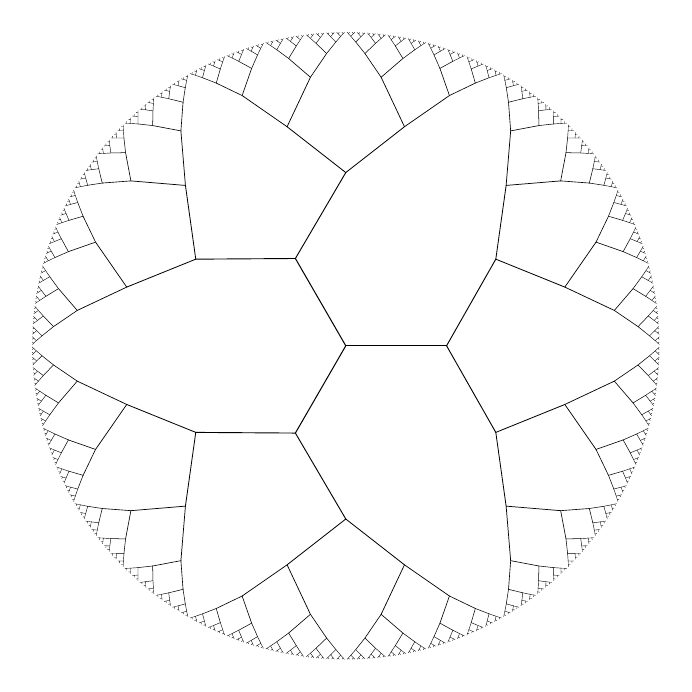
\begin{tikzpicture}[
  x=\ArbolTresRegularEscala,y=\ArbolTresRegularEscala,
  draw=black,line cap=round,line join=round]
  \path[use as bounding box] (-1.01,-1.01) rectangle (1.01,1.01);
  % Argumentos: nivel, angulo central, semiancho del sector, x e y del padre.
  \def\arboltresrama#1#2#3#4#5{%
    \begingroup
    \ifnum#1=1\relax
      \def\arboltresradio{.32}%
    \else\ifnum#1=2\relax
      \def\arboltresradio{.55}%
    \else
      \pgfmathsetmacro{\arboltresradio}{1-.28*pow(.5,#1-3)}%
    \fi\fi
    \pgfmathsetmacro{\arboltresx}{\arboltresradio*cos(#2)}%
    \pgfmathsetmacro{\arboltresy}{\arboltresradio*sin(#2)}%
    \pgfmathsetmacro{\arboltresgrosor}{max(.12,.4-.035*#1)}%
    \draw[line width=\arboltresgrosor pt] (#4,#5)--(\arboltresx,\arboltresy);
    \ifnum#1<\ArbolTresRegularNiveles\relax
      \pgfmathtruncatemacro{\arboltresnivel}{#1+1}%
      \pgfmathsetmacro{\arboltressector}{#3/2}%
      \foreach \arboltressigno in {-1,1}{%
        \pgfmathsetmacro{\arboltresangulo}{#2+\arboltressigno*\arboltressector}%
        \edef\arboltresllamada{\noexpand\arboltresrama
          {\arboltresnivel}{\arboltresangulo}{\arboltressector}{\arboltresx}{\arboltresy}}%
        \arboltresllamada
      }%
    \else
      % Cada extremo continua ramificandose indefinidamente.
      \pgfmathsetmacro{\arboltresfinal}{1-.28*pow(.5,#1-2)}%
      \foreach \arboltressigno in {-1,1}{%
        \pgfmathsetmacro{\arboltresangulo}{#2+\arboltressigno*#3/2}%
        \draw[line width=.12pt]
          (\arboltresx,\arboltresy)--(\arboltresangulo:\arboltresfinal);
      }%
    \fi
    \endgroup
  }
  \arboltresrama{1}{0}{60}{0}{0}
  \arboltresrama{1}{120}{60}{0}{0}
  \arboltresrama{1}{240}{60}{0}{0}
\end{tikzpicture}
\endgroup

% Opcional, antes de \input: \def\ArbolTresRegularNiveles{8}
%                           \def\ArbolTresRegularEscala{4cm}
% La raiz tiene tres hijos a 120 grados; los demas vertices tienen dos hijos.
% Las bifurcaciones de la periferia representan la continuacion infinita.
% No se dibuja una circunferencia de cierre, que introduciria ciclos.
\begingroup
\providecommand{\ArbolTresRegularNiveles}{8}
\providecommand{\ArbolTresRegularEscala}{4cm}
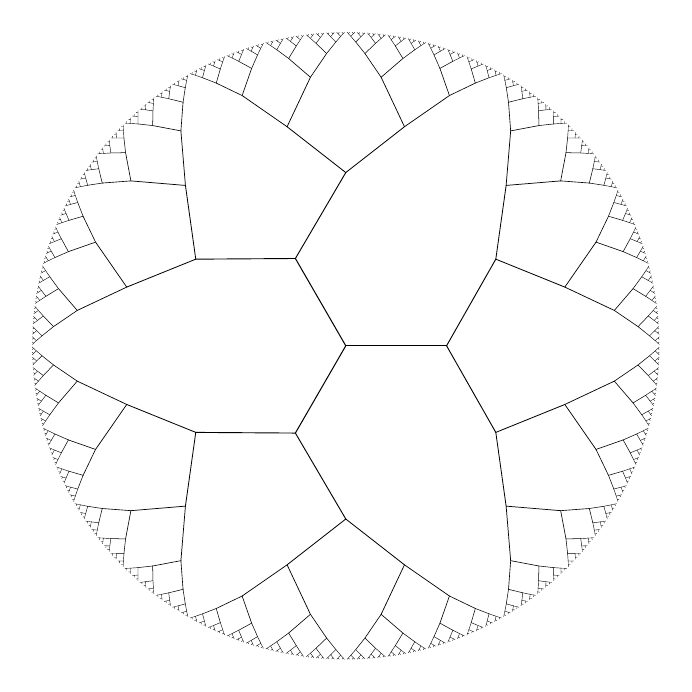
\begin{tikzpicture}[
  x=\ArbolTresRegularEscala,y=\ArbolTresRegularEscala,
  draw=black,line cap=round,line join=round]
  \path[use as bounding box] (-1.01,-1.01) rectangle (1.01,1.01);
  % Argumentos: nivel, angulo central, semiancho del sector, x e y del padre.
  \def\arboltresrama#1#2#3#4#5{%
    \begingroup
    \ifnum#1=1\relax
      \def\arboltresradio{.32}%
    \else\ifnum#1=2\relax
      \def\arboltresradio{.55}%
    \else
      \pgfmathsetmacro{\arboltresradio}{1-.28*pow(.5,#1-3)}%
    \fi\fi
    \pgfmathsetmacro{\arboltresx}{\arboltresradio*cos(#2)}%
    \pgfmathsetmacro{\arboltresy}{\arboltresradio*sin(#2)}%
    \pgfmathsetmacro{\arboltresgrosor}{max(.12,.4-.035*#1)}%
    \draw[line width=\arboltresgrosor pt] (#4,#5)--(\arboltresx,\arboltresy);
    \ifnum#1<\ArbolTresRegularNiveles\relax
      \pgfmathtruncatemacro{\arboltresnivel}{#1+1}%
      \pgfmathsetmacro{\arboltressector}{#3/2}%
      \foreach \arboltressigno in {-1,1}{%
        \pgfmathsetmacro{\arboltresangulo}{#2+\arboltressigno*\arboltressector}%
        \edef\arboltresllamada{\noexpand\arboltresrama
          {\arboltresnivel}{\arboltresangulo}{\arboltressector}{\arboltresx}{\arboltresy}}%
        \arboltresllamada
      }%
    \else
      % Cada extremo continua ramificandose indefinidamente.
      \pgfmathsetmacro{\arboltresfinal}{1-.28*pow(.5,#1-2)}%
      \foreach \arboltressigno in {-1,1}{%
        \pgfmathsetmacro{\arboltresangulo}{#2+\arboltressigno*#3/2}%
        \draw[line width=.12pt]
          (\arboltresx,\arboltresy)--(\arboltresangulo:\arboltresfinal);
      }%
    \fi
    \endgroup
  }
  \arboltresrama{1}{0}{60}{0}{0}
  \arboltresrama{1}{120}{60}{0}{0}
  \arboltresrama{1}{240}{60}{0}{0}
\end{tikzpicture}
\endgroup

% Opcional, antes de \input: \def\ArbolTresRegularNiveles{8}
%                           \def\ArbolTresRegularEscala{4cm}
% La raiz tiene tres hijos a 120 grados; los demas vertices tienen dos hijos.
% Las bifurcaciones de la periferia representan la continuacion infinita.
% No se dibuja una circunferencia de cierre, que introduciria ciclos.
\begingroup
\providecommand{\ArbolTresRegularNiveles}{8}
\providecommand{\ArbolTresRegularEscala}{4cm}
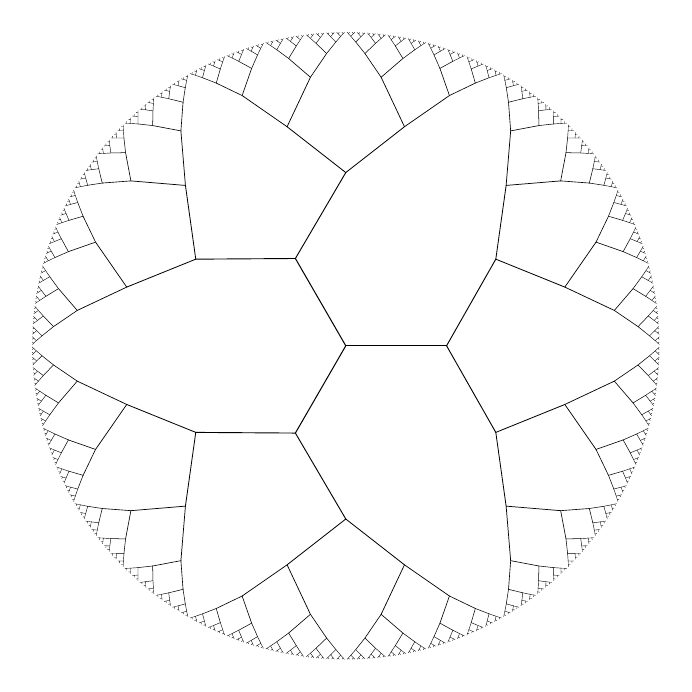
\begin{tikzpicture}[
  x=\ArbolTresRegularEscala,y=\ArbolTresRegularEscala,
  draw=black,line cap=round,line join=round]
  \path[use as bounding box] (-1.01,-1.01) rectangle (1.01,1.01);
  % Argumentos: nivel, angulo central, semiancho del sector, x e y del padre.
  \def\arboltresrama#1#2#3#4#5{%
    \begingroup
    \ifnum#1=1\relax
      \def\arboltresradio{.32}%
    \else\ifnum#1=2\relax
      \def\arboltresradio{.55}%
    \else
      \pgfmathsetmacro{\arboltresradio}{1-.28*pow(.5,#1-3)}%
    \fi\fi
    \pgfmathsetmacro{\arboltresx}{\arboltresradio*cos(#2)}%
    \pgfmathsetmacro{\arboltresy}{\arboltresradio*sin(#2)}%
    \pgfmathsetmacro{\arboltresgrosor}{max(.12,.4-.035*#1)}%
    \draw[line width=\arboltresgrosor pt] (#4,#5)--(\arboltresx,\arboltresy);
    \ifnum#1<\ArbolTresRegularNiveles\relax
      \pgfmathtruncatemacro{\arboltresnivel}{#1+1}%
      \pgfmathsetmacro{\arboltressector}{#3/2}%
      \foreach \arboltressigno in {-1,1}{%
        \pgfmathsetmacro{\arboltresangulo}{#2+\arboltressigno*\arboltressector}%
        \edef\arboltresllamada{\noexpand\arboltresrama
          {\arboltresnivel}{\arboltresangulo}{\arboltressector}{\arboltresx}{\arboltresy}}%
        \arboltresllamada
      }%
    \else
      % Cada extremo continua ramificandose indefinidamente.
      \pgfmathsetmacro{\arboltresfinal}{1-.28*pow(.5,#1-2)}%
      \foreach \arboltressigno in {-1,1}{%
        \pgfmathsetmacro{\arboltresangulo}{#2+\arboltressigno*#3/2}%
        \draw[line width=.12pt]
          (\arboltresx,\arboltresy)--(\arboltresangulo:\arboltresfinal);
      }%
    \fi
    \endgroup
  }
  \arboltresrama{1}{0}{60}{0}{0}
  \arboltresrama{1}{120}{60}{0}{0}
  \arboltresrama{1}{240}{60}{0}{0}
\end{tikzpicture}
\endgroup
\\[1.2cm]
{\Large\bfseries Docente:}\\[.2cm]
{\Large\Docente}\\[.5cm]
{\Large\bfseries Alumno:}\\[.2cm]
{\Large\Alumno}
\end{center}
\end{titlepage}
\restoregeometry
